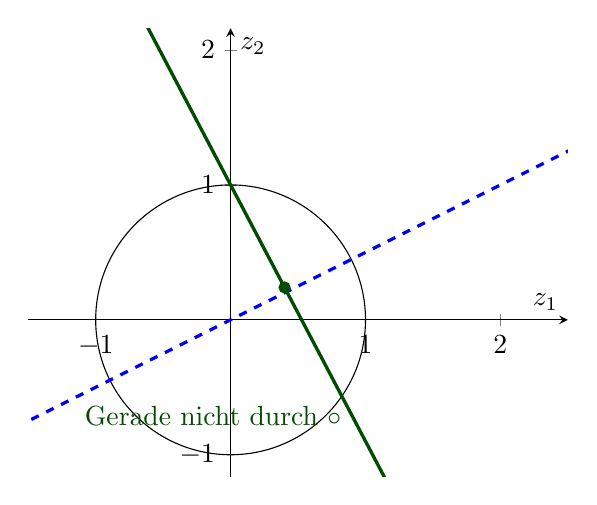
\begin{tikzpicture}
	\begin{axis}[
		axis lines=middle,
		axis equal,
		xmin=-1.5,
		xmax=2.5,
		ymin=-1,
		ymax=2,
		xlabel=$z_1$,
		ylabel=$z_2$,
		]	
		\draw (axis cs: 0, 0) circle [radius=1];
		\addplot[-, blue, very thick, dashed] {0.5*x};
		\addplot[-, black!70!green, very thick] {-1.9*x + 1} node[above, left, black!70!green, pos=0.59] {Gerade nicht durch $\circ$};
		\addplot[mark=*, black!70!green] coordinates {(0.4, 0.24)};
	\end{axis}
\end{tikzpicture}